%%%%%%%%%%%%%%%%%%%%%%%%%%%%%%%%%%%%%%%%%%%%%%%%%%%%%%%%%%%%%%%%%%%
%%%%%%%%%%%%%%%%%%%%%%%%%%%%%%%%%%%%%%%%%%%%%%%%%%%%%%%%%%%%%%%%%%%
\section{Introdução} % Sections can be created in order to organize your presentation into discrete blocks, all sections and subsections are automatically printed in the table of contents as an overview of the talk

%%%%%%%%%%%%%%%%%%%%%%%%%%%%%%%%%%%%%%%%%%%%%%%%%%%%%%%%%%%%%%%%%%%
\subsection{Agricultura de precisão}

\begin{frame}
\frametitle{Agricultura de precisão}
\end{frame}

%%%%%%%%%%%%%%%%%%%%%%%%%%%%%%%%%%%%%%%%%%%%%%%%%%%%%%%%%%%%%%%%%%%
\subsection{GPS}

\begin{frame}
\frametitle{GPS}
\end{frame}

%%%%%%%%%%%%%%%%%%%%%%%%%%%%%%%%%%%%%%%%%%%%%%%%%%%%%%%%%%%%%%%%%%%
\subsection{Microcontrolador}

\begin{frame}
\frametitle{Microcontrolador}
\end{frame}





%%%%%%%%%%%%%%%%%%%%%%%%%%%%%%%%%%%%%%%%%%%%%%%%%%%%%%%%%%%%%%%%%%%%%%%%%%%%%%%%%
%%%%%%%%%%%%%%%%%%%%%%%%%%%%%%%%%%%%%%%%%%%%%%%%%%%%%%%%%%%%%%%%%%%%%%%%%%%%%%%%

\section{Plano de estágio}

\subsection{A Empresa}

\begin{frame}%[noframenumbering]
\frametitle{A empresa}
\begin{columns}

	\column{0.7\linewidth}
	\begin{figure}[]
	 \centering
	 \captionsetup{width=\textwidth,font=footnotesize,textfont=bf}
	 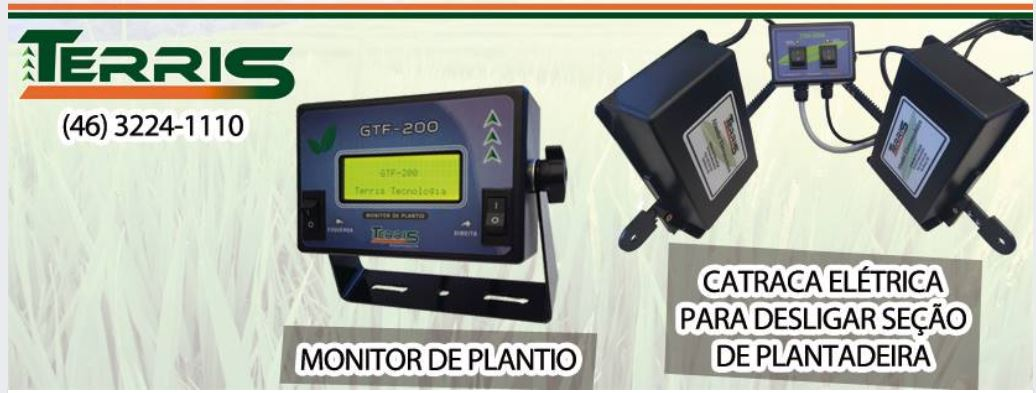
\includegraphics[width=\textwidth,keepaspectratio]{Figuras/Terris.jpg}
	 \caption{Logo da Terris}
	\end{figure}
	
	\column{0.4\linewidth}
	\begin{itemize}
	\item Terris automação agrícola
	\pause
	\item Empresa encubada
	\pause
	\item Produtos desenvolvidos e comercializados
	\end{itemize}

\end{columns}
\end{frame}

%%%%%%%%%%%%%%%%%%%%%%%%%%%%%%%%%%%%%%%%%%%%%%%%%%%%%%%%%%%%%%%%%%%%%%
\subsection{O Estágio}

\begin{frame}
\frametitle{O Estágio}

\begin{itemize}
	\item \textbf{Área de atuação}: Pesquisa e desenvolvimento
	\pause
	\item \textbf{Tipo de estágio}: Estudo dirigido
	\pause
	\item \textbf{Setor da empresa}: Pesquisa e desenvolvimento
	\pause	
	\item \textbf{Orientador(a)}: Professora Dra. Beatriz Terezinha Borsoi
	\pause
	\item \textbf{Contatos na empresa}: \\Sidney Gaspari\\ Josimar Tumeleiro
\end{itemize}
\end{frame}

%%%%%%%%%%%%%%%%%%%%%%%%%%%%%%%%%%%%%%%%%%%%%%%%%%%%%%%%%%%%%%%%%%%%%%%%%%%%%
%\subsection{Atividade desenvolvida}
\begin{frame}
\frametitle{O Estágio}

\begin{block}{Atividade desenvolvida}
\begin{itemize}
\item Estudo comparativo entre os módulos \textit{Global Position System} (GPS), ou Sistema de Posicionamento Global, verificando a sua aplicabilidade na agricultura de precisão.
\pause 
\item Programação dos sensores utilizando o microcontrolador STM32F030R8, da STMicroelectronics\textregistered, visando a aplicação dos módulos estudados em um produto comercial desenvolvida pela empresa Terris\textregistered, que trabalha com o desenvolvimento de tecnologias agrícolas.
\end{itemize}
\end{block}

\end{frame}


%%%%%%%%%%%%%%%%%%%%%%% EOF %%%%%%%%%%%%%%%%%%%%%%%%%%%%